\documentclass[12pt]{article}

\usepackage{scicite,times,graphicx,float,hyperref}
\usepackage[skip=0pt]{caption}
\usepackage[utf8]{inputenc}

\topmargin -1.0cm
\oddsidemargin 0.0cm
\textwidth 16cm 
\textheight 23cm
\footskip 1.0cm

\newenvironment{sciabstract}{%
\begin{quote} \bf}
{\end{quote}}

\newcounter{lastnote}
\newenvironment{scilastnote}{%
  \setcounter{lastnote}{\value{enumiv}}%
  \addtocounter{lastnote}{+1}%
  \begin{list}%
  {\arabic{lastnote}.}
  {\setlength{\leftmargin}{.22in}}
  {\setlength{\labelsep}{.5em}}
}
{\end{list}}

\title{Lab Work 3} 

\author
{André Pedrosa [85098], Filipe Pires [85122], João Alegria [85048]\\
\\
Algorithmic Information Theory\\
\normalsize{Department of Electronics, Telecommunications and Informatics}\\
\normalsize{University of Aveiro}\\
} 

\date{\today{}}

%%%%%%%%%%%%%%%%% END OF PREAMBLE %%%%%%%%%%%%%%%%

\begin{document} 

\baselineskip18pt

\maketitle 

\section{Introduction} %%%%%%%%%%%%%%%%%%%%%%%%%%%%%%%%%%%%%%%%%%%%%%%%%%%%%%%%%%%%%%%%%%%%%%%%%%%%%%%%%%%%%%%%%%%%%%%%%%%%%%%%%%%%%%%%%%%%%%%%%%%%%%%%%%%%%%%%%

This report aims to describe the work developed for the third and final assignment of the course of 'Algorithmic Information Theory', explaining all scripts
developed by us and presenting the results we considered most relevant regarding the quality of the solutions. 

The programs implemented in Shell have the purpose of measuring similarity of images using a compression-based strategy and automatically identify human faces.
Along with the description of the solutions, we also discuss the characteristics and the preprocessing done to the available dataset, the data compression 
algorithms used and the tests executed.
All code developed is publicly accessible in our GitHub repository: 

\url{https://github.com/joao-alegria/TAI}.
\newpage

\section{Image Classification} %%%%%%%%%%%%%%%%%%%%%%%%%%%%%%%%%%%%%%%%%%%%%%%%%%%%%%%%%%%%%%%%%%%%%%%%%%%%%%%%%%%%%%%%%%%%%%%%%%%%%%%%%%%%%%%%%%%%%%%%%%%%%%%%%

When dealing with image processing problems that require object identification, the usual environment calls for a classification approach, as the objects to 
be identified belong to specific classes with clear and separable characteristics.
The challenge we are faced with \cite{trab3} is a special approach for the image classification problem of facial recognition or identification.
It is special in the sense that it does not aim to explore the usual strategies based on feature extraction, rather it is meant to rely on data compression 
methods and the notion of algorithmic information.
Algorithmic information, also known as algorithmic entropy or Kolmogorov complexity, is the measure of information in a given data portion based on the 
theoretical algorithm that would be required to recreate that same data portion. 

As this is an abstract definition, an example can clarify the concept: 
considering strings A="0101010101" and B="0010100110", for instance, one can easily reach the conclusion that string A is far easier to define than string B,
since for A we can simply define it as the smaller string "01" repeated 5 times; string B, on the other hand, the process is not as simple and we probably will
require the entire string to describe it.
What this means is that A has less information than B. 
To achieve the so called algorithmic information of each one, the thought process is the same but now the string descriptions are achieved through algorithms;
for our examples, the algorithms that define strings A and B are the following: 

\vspace{0.2in}
\begin{minipage}{0.45\textwidth}
  \begin{verbatim}
    def stringA():
      for i in range(5):
        print("01", end="")
  \end{verbatim}
\end{minipage}
\begin{minipage}{0.45\textwidth}
  \begin{verbatim}
    def stringB():
      for letter in "0010100110":
        print(letter, end="")
  \end{verbatim}
\end{minipage}
\vspace{0.2in}

By a quick analysis, it is obvious that \textit{stringA()} is less complex than \textit{stringB()}, iterating only 5 times, contrasting with the 10 iterations 
of the second; hence confirming that string B has more information than string A. 
This can be directly correlated with data compression, since compressors take advantage of the data repetition to reduce space usage, and thereby compress the 
information by storing the data that appears frequently and the indicators of the places where those repetitions occur.

With this in mind, one can proceed to understand how the image classification will be done. 
Using the Normalized Information Distance defined by equation \ref{eq:1}, where \textit{K(x)} and \textit{K(x|y)} define the Kolmogorov complexity of the 
string $x$ and of the string $x$ given string $y$. 

\begin{equation} \label{eq:1}
  NID(x,y) = \frac{max\{K(x|y),K(y|x)\}}{max\{K(x),K(y)\}}
\end{equation}
\newpage

Unfortunately, because the Kolmogorov complexity is non-computable, this formula is only theoretical and we are sure there is no algorithm that can compute 
any string complexity. 
Nevertheless, compressors approximate the formula's results very closely, if used correctly. 
So we used two of the most frequently used approximations of \texttt{NID} to determine the compression distance between images and, with these distances, 
calculate the closest images, i.e. the most similar ones, and hopefully classify them as belonging to the group of images that represent the same face.

\subsection{NCD Approximation} %%%%%%%%%%%%%%%%%%%%%%%%%%%%%%%%%%%%%%%%%%%%%%%%%%%%%%%%%%%

By using known general purpose compressors, such as gzip, lzma, tar, ..., the Kolmogorov complexity can be estimated by the number of bits the resulting compressed file has. 
This approximation is expressed by equation \ref{eq:2}, where \textit{C(x)} and \textit{C(x,y)} represent the number of bits the compression of $x$ and of 
$x$ and $y$ concatenated contain, respectively.
The $xy$ concatenation can be performed in several ways, the most common being to simply perform an union on both; other more complex operations can also be done, 
such as interlacing the two data sources. 

\begin{equation}\label{eq:2}
  NCD(x,y) = \frac{C(x,y)-min\{C(x), C(y)\}}{max\{C(x),C(y)\}}
\end{equation}

Following the formula, results close to 0 indicate similarity and close to 1 dissimilarity. The only restriction to this approach is that the compressor used must follow the condition $C(x,x) \simeq C(x)$, without that the results of NCD may not be reliable nor true. 


\subsection{NCCD Approximation} %%%%%%%%%%%%%%%%%%%%%%%%%%%%%%%%%%%%%%%%%%%%%%%%%%%%%%%%%%

This approach is yet another approximation to the NID formula, this time using conditional compressors to achieve their estimation. Conditional compressors are normally implemented with finite-context models and take in consideration the previous occurring terms to compress the new term. This is a more direct approximation of the NID and, in general, generate better results than the NCD. Defined by:

\begin{equation}\label{eq:3}
  NCCD(x,y) = \frac{max\{C(x|y), C(y|x)\}}{max\{C(x), C(y)\}}
\end{equation}

Where \textit{C(x)} defines once again the number of bits the compression of the object x by a given conditional compressor and $C(x|y)$ represents the number of bits the compression of x needs given that y occurred previously ($C(y|x)$ has the same logic). Due to the consitional aspect of this approach, \textit{C(x)} can be a special case of $C(x|y)$ were y is equal to the empty string, causing that $C(x) = C(x|\epsilon)$.

\newpage
\section{Dataset} %%%%%%%%%%%%%%%%%%%%%%%%%%%%%%%%%%%%%%%%%%%%%%%%%%%%%%%%%%%%%%%%%%%%%%%%%%%%%%%%%%%%%%%%%%%%%%%%%%%%%%%%%%%%%%%%%%%%%%%%%%%%%%%%%%%%%%%%%%%%%%

Like in all experimental work, specially in image processing, a considerably large dataset is required for any results to be significant and any conclusions to be solid.
Also, when benchmarking an algorithm, it is recommended that standard test datasets are used for researchers to be able to directly compare the results. 
Taking this in consideration, we downloaded AT\&T "The Database of Faces" (formerly "The ORL Database of Faces") and used it to test our code.

The image database contains 10 different images of each of the 40 distinct subjects.
For some subjects the images were taken at different times, between April 1992 and April 1994, with varying lighting conditions and different facial expressions.
Most faces are in an upright position in frontal view, with a slight left-right rotation.
All 400 images were taken in black \& white at the Olivetti Research Laboratory in Cambridge, UK.

\begin{figure}[H]
  \centering
  \begin{minipage}{\textwidth}
    \centering
    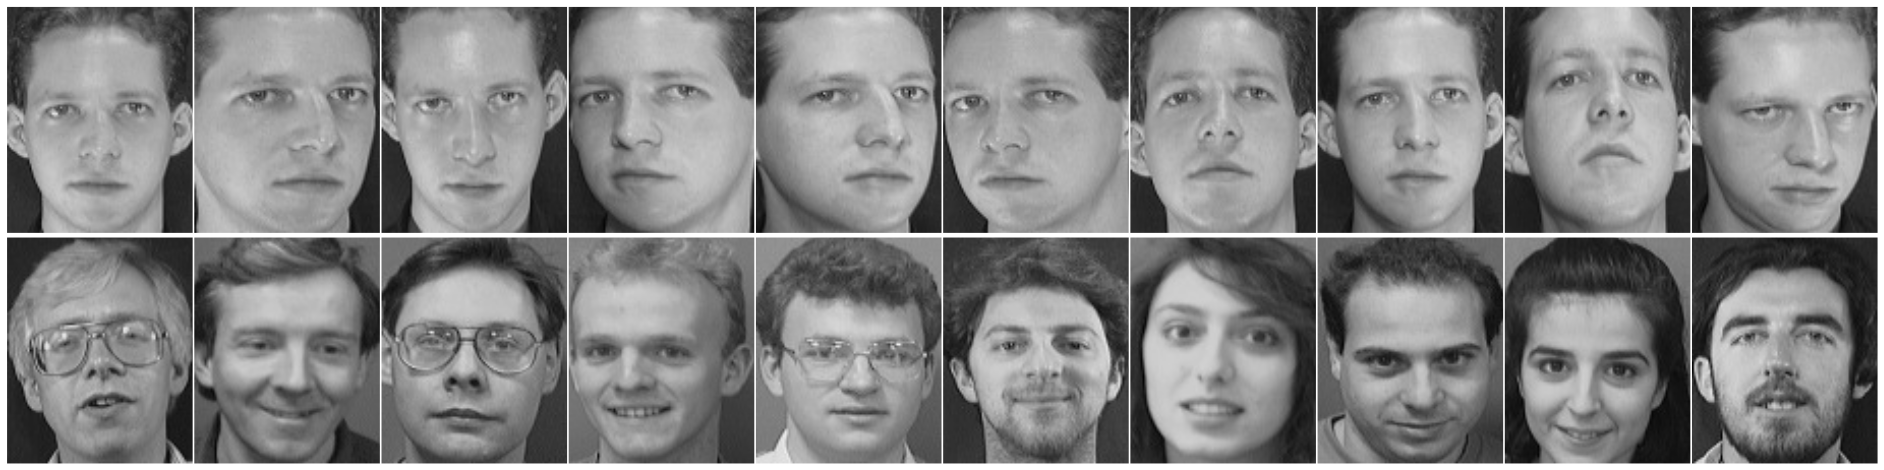
\includegraphics[width=\linewidth]{faces_example.png}
  \end{minipage}%
  \caption{Image taken from the assignment description \cite{trab3}. Examples from the ORL face dataset. In the first row, ten face images corresponding to the same subject (s01). In the second row, the first face image of subjects s02 to s11.}
  \label{fig:quantization}
\end{figure}

To speedup the processing of each image, we applied 2 transformations to each element of the dataset.
The first consisted in a simple image reduction from 112 $\times$ 92 px to 56 $\times$ 46 px, ensuring that proportions remained the same.
The second was a quantization process from 8 bits per pixel gray level to 4 bits only.
These modifications were accomplished using ImageMagick \cite{imgmagick}, a command-line program to create, edit, compose, or convert bitmap images.

\begin{figure}[H]
  \centering
  \begin{minipage}{.2\textwidth}
    \centering
    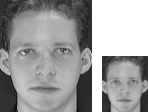
\includegraphics[width=\linewidth]{preprocessing_example.png}
  \end{minipage}%
  \caption{Example from subject s01 of the ORL face dataset, before and after preprocessing.}
  \label{fig:quantization}
\end{figure}

\newpage
\section{Experiment} %%%%%%%%%%%%%%%%%%%%%%%%%%%%%%%%%%%%%%%%%%%%%%%%%%%%%%%%%%%%%%%%%%%%%%%%%%%%%%%%%%%%%%%%%%%%%%%%%%%%%%%%%%%%%%%%%%%%%%%%%%%%%%%%%%%%%%%%%%%
Lorem ipsum ...

\subsection{Tested Compressors}%%%%%%%%%%%%%%%%%%%%%%%%%%%%%%%%%%%%%%%%%%%%%%%%%%%%%%%%%%%
.......

\section{Results \& Discussion} %%%%%%%%%%%%%%%%%%%%%%%%%%%%%%%%%%%%%%%%%%%%%%%%%%%%%%%%%%%%%%%%%%%%%%%%%%%%%%%%%%%%%%%%%%%%%%%%%%%%%%%%%%%%%%%%%%%%%%%%%%%%%%%%
Lorem ipsum ...


\section{Conclusions} %%%%%%%%%%%%%%%%%%%%%%%%%%%%%%%%%%%%%%%%%%%%%%%%%%%%%%%%%%%%%%%%%%%%%%%%%%%%%%%%%%%%%%%%%%%%%%%%%%%%%%%%%%%%%%%%%%%%%%%%%%%%%%%%%%%%%%%%%%

After completing the assignment, we drew a few conclusions regarding our 
solutions and ..................

Lorem ipsum ...

In terms of code organization and readability, we made sure our 
repository was as well structured as possible and our code properly commented
and documented.
The base folder contains a {\it README\/} file for basic instructions.
All code is in the {\it src\/} folder.

\newpage
\begin{thebibliography}{9} %%%%%%%%%%%%%%%%%%%%%%%%%%%%%%%%%%%%%%%%%%%%%%%%%%%%%%%%%%%%%%%%%%%%%%%%%%%%%%%%%%%%%%%%%%%%%%%%%%%%%%%%%%%%%%%%%%%%%%%%%%%%%%%%%%%%%
  \bibliographystyle{Science}

  \bibitem{trab3}
    Armando J. Pinho,
    \textit{AIT: Lab Work no.3},
    University of Aveiro,
    2019/20.
  
  \bibitem{imgmagick}
    ImageMagick Studio LLC,
    \textit{ImageMagick},
    \url{https://imagemagick.org/index.php},
    accessed in December 2019.
  
\end{thebibliography}

\clearpage

\end{document}




















